\documentclass[a4paper]{iacas}

\usepackage{cite}
\usepackage{hyperref}% embedding hyperlinks [must be loaded after dropping]
\usepackage{amsmath,amsthm,amssymb,amsfonts,latexsym,mathrsfs,wasysym}
\usepackage{marvosym}
\usepackage{subcaption}
\usepackage{soul,color}
\usepackage{threeparttable}% tables with footnotes
\usepackage{dcolumn}% decimal-aligned tabular math columns
\usepackage{float}
\usepackage{graphicx}
\usepackage{accents}
\usepackage{tikz}
\usepackage{lastpage}
\usepackage{fancyhdr}
\usepackage{color}
\usepackage{cancel}
\usepackage{setspace}
%\doublespacing
% or:
\onehalfspacing
%\usepackage[T1]{fontenc}
%\usepackage{bigfoot} % to allow verbatim in footnote
\usepackage[framed,numbered]{matlab-prettifier}
\pagestyle{plain}
%\usepackage[hebrew,english]{babel}
\usetikzlibrary{shapes.geometric, arrows, calc}

\newcolumntype{d}{D{.}{.}{-1}}
\graphicspath{{figures/}}

% define some commands to maintain consistency
\newcommand{\pkg}[1]{\texttt{#1}}
\newcommand{\cls}[1]{\textsf{#1}}
\newcommand{\file}[1]{\texttt{#1}}
\newcommand{\sgn}[1]{\operatorname{sgn}\left(#1\right)}
\newcommand{\sat}[1]{\operatorname{sat}\left(#1\right)}
\newcommand{\rrule}[1]{\rule[#1]{0pt}{0pt}}
\newcommand{\fracds}[2]{\frac{\displaystyle #1\rrule{-0.2em}}{\displaystyle #2\rrule{1em}}}
\newcommand{\figref}[1]{Fig.~\ref{#1}}
\newcommand{\ubar}[1]{\underaccent{\bar}{#1}}
\newcommand{\norm}[1]{\lvert \lvert \vec #1 \rvert \rvert}

%diffeomorphism

\begin{document}


%\begin{tabular}{l}
%\\
%{\bf\textit{Alexander Shender 328626114}} \\
%{\bf\textit{Vladimir Tchuiev 309206795}} \\
%Technion - Israel Institute of Technology
%\end{tabular}

\vspace{2em}

\section{Image Stitching Section}

\subsection{Step 1}

We extracted sift features from interest points from all images in Fig.~\ref{fig:100}. The images with more details contain more interest points including the sky gradients. Those interest points will be discarded when matching those points.

\begin{figure}[!htbp]
	
	\begin{subfigure}[b]{0.23\textwidth}
		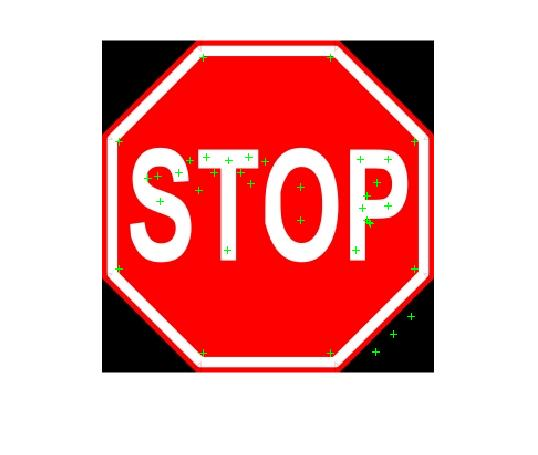
\includegraphics[width=\textwidth]{101.jpg}
		\caption{}
		\label{fig:101}
	\end{subfigure}
	%
	\begin{subfigure}[b]{0.23\textwidth}
		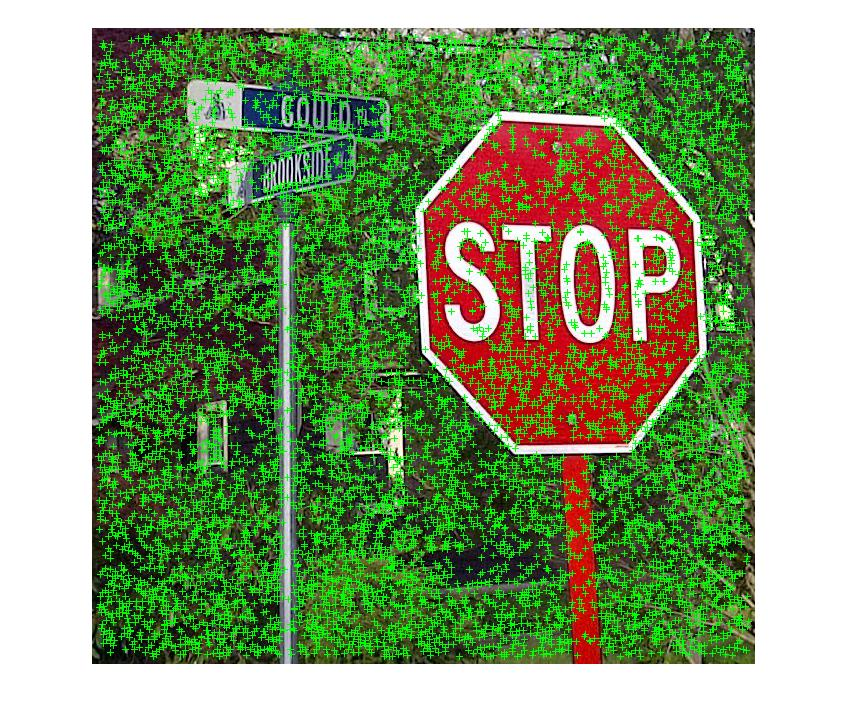
\includegraphics[width=\textwidth]{102.jpg}
		\caption{}
		\label{fig:102}
	\end{subfigure}
	%
	\begin{subfigure}[b]{0.23\textwidth}
		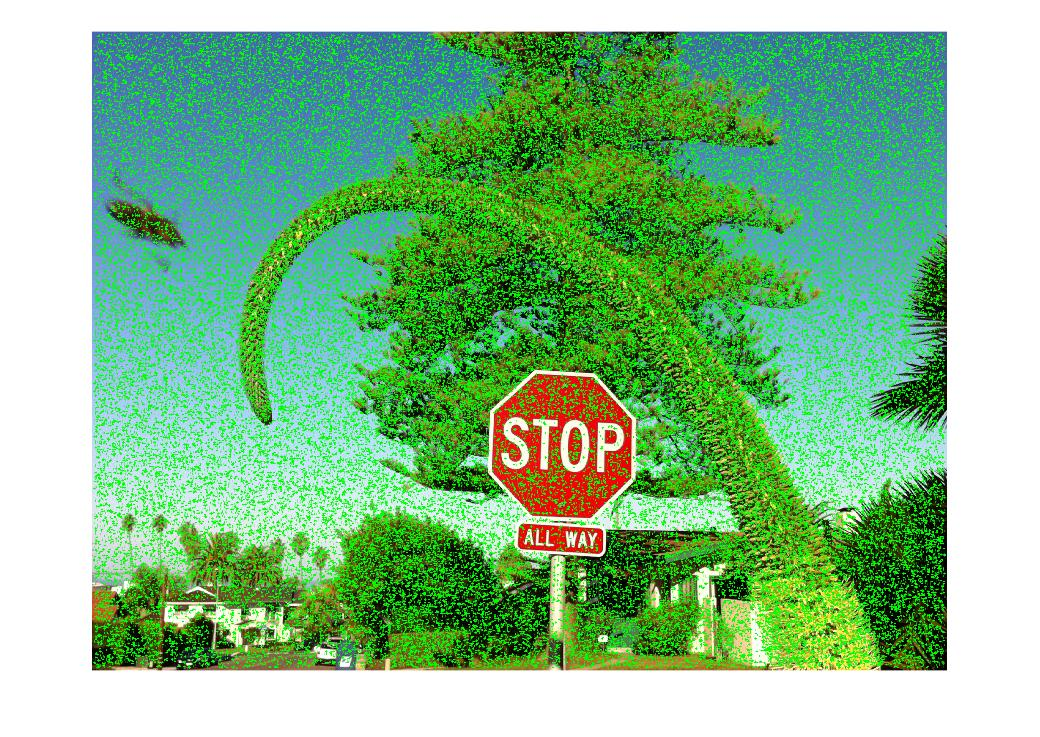
\includegraphics[width=\textwidth]{103.jpg}
		\caption{}
		\label{fig:103}
	\end{subfigure}
	%
	\begin{subfigure}[b]{0.23\textwidth}
		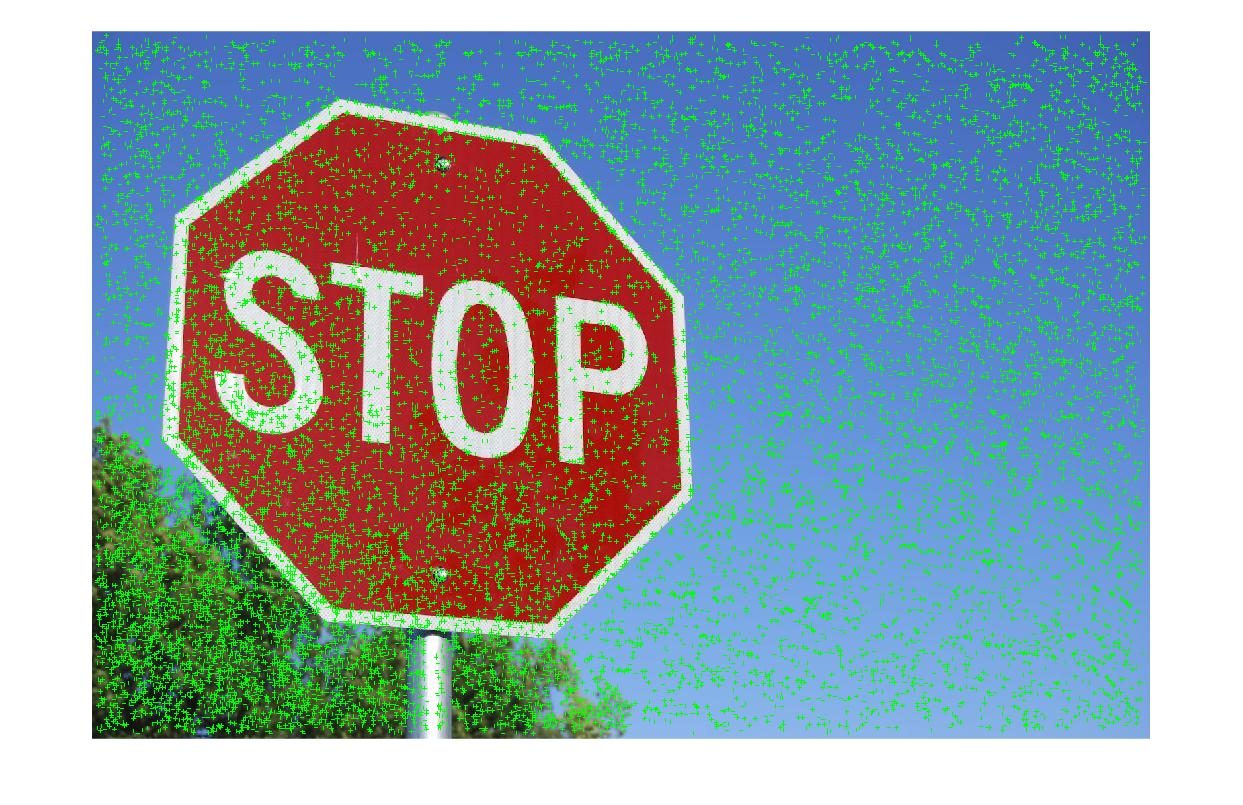
\includegraphics[width=\textwidth]{104.jpg}
		\caption{}
		\label{fig:104}
	\end{subfigure}
	
	\caption{Sift feature points for each Stop sign image, each point presented as a green cross.}
	\label{fig:100}
\end{figure}

\subsection{Step 2}

Using the \textit{siftmatch} function we do a preliminary match between similar sift features in image 1 to all the rest (Fig.~\ref{fig:200}). While generally the SIFT match is good, there are visible outliers created by this algorithm (especially visible in Fig.~\ref{fig:202}), outliers that will be cleaned next.

\begin{figure}[!htbp]
	
	\begin{subfigure}[b]{0.32\textwidth}
		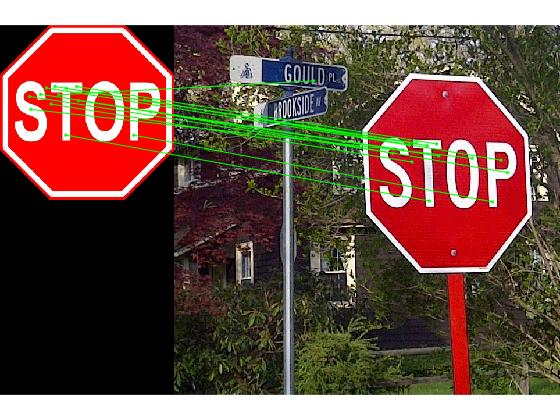
\includegraphics[width=\textwidth]{202.jpg}
		\caption{}
		\label{fig:202}
	\end{subfigure}
	%
	\begin{subfigure}[b]{0.32\textwidth}
		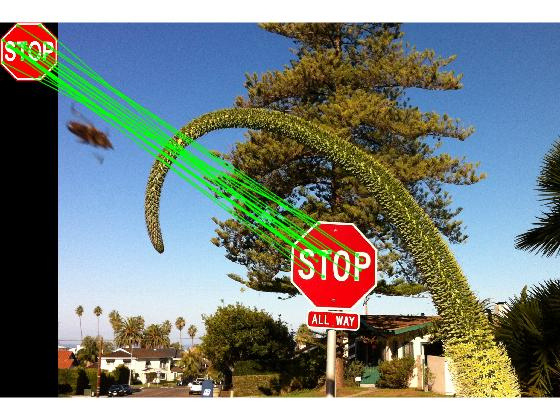
\includegraphics[width=\textwidth]{203.jpg}
		\caption{}
		\label{fig:203}
	\end{subfigure}
	%
	\begin{subfigure}[b]{0.32\textwidth}
		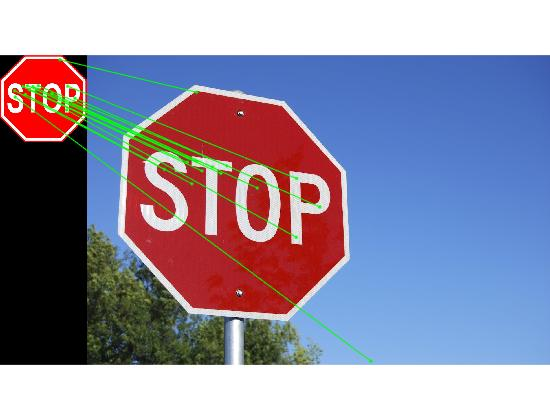
\includegraphics[width=\textwidth]{204.jpg}
		\caption{}
		\label{fig:204}
	\end{subfigure}
	
	\caption{Sift feature matching between images and the nominal Stop sign, green lines connect between matching features.}
	\label{fig:200}
\end{figure}

\subsection{Step 3}

The next step is to perform RANSAC to weed out the outliers and find the affine transformation matrices from all the inliers. Eq.~\ref{eq:Affine Matrices} presents all the affine matrices, where $H_i$ is the transformation matrix between image 1 and image $i$. As a requirement, perspective distortion wasn't considered, and the effect will be evident in a later section where the stitching is not aligned perfectly with one of the images.

\begin{equation}
\tiny
H_2 = \left[
\begin{array}{ccc}
0.9382 & 0.0487 & 322.1 \\
0.0193 & 1.1876 & 74.0131 \\
0 & 0 & 1
\end{array}
\right]
\quad H_3 = \left[
\begin{array}{ccc}
1.4661 & -0.047 & 1212 \\
0.053 & 1.5614 & 1011 \\
0 & 0 & 1
\end{array}
\right]
\quad H_4 = \left[
\begin{array}{ccc}
2.613 & -0.1745 & 154.9 \\
0.3577 & 2.564 & 59.74 \\
0 & 0 & 1
\end{array}
\right]
\end{equation}\label{eq:Affine Matrices}

\subsection{Step 4}

In this step, we present the interest point matches using both SIFT feature similarity and RANSAC outlier filtering in Fig.~\ref{fig:400}. We see most of the interest points were preserved and all the obvious outliers removed, in particular compare between Fig.~\ref{fig:402} and Fig.~\ref{fig:202}, where the obvious horizontal outlier was removed.

\begin{figure}[!htbp]
	
	\begin{subfigure}[b]{0.32\textwidth}
		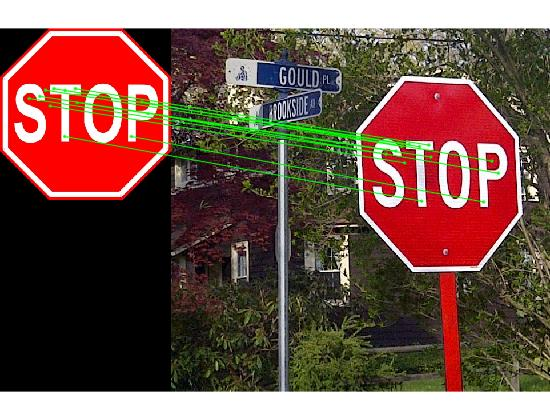
\includegraphics[width=\textwidth]{402.jpg}
		\caption{}
		\label{fig:402}
	\end{subfigure}
	%
	\begin{subfigure}[b]{0.32\textwidth}
		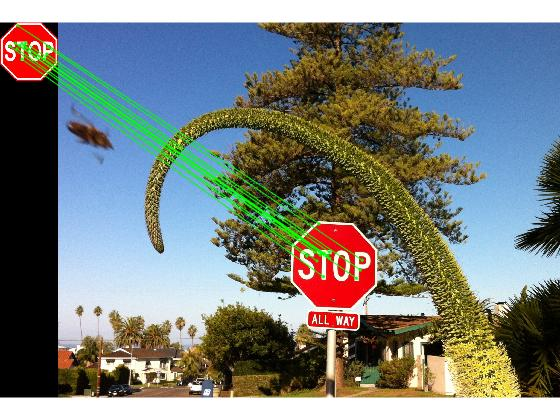
\includegraphics[width=\textwidth]{403.jpg}
		\caption{}
		\label{fig:403}
	\end{subfigure}
	%
	\begin{subfigure}[b]{0.32\textwidth}
		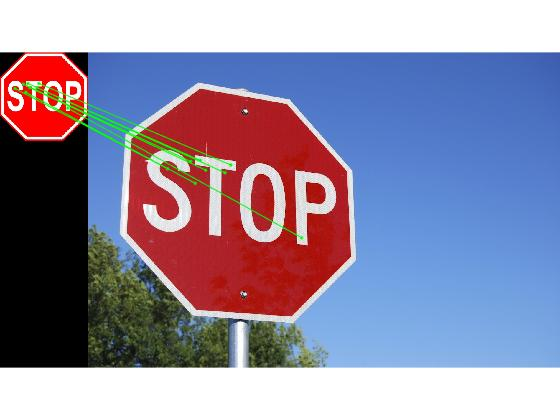
\includegraphics[width=\textwidth]{404.jpg}
		\caption{}
		\label{fig:404}
	\end{subfigure}
	
	\caption{Matching features after RANSAC with the most inliers.}
	\label{fig:400}
\end{figure}

\subsection{Step 5}

In this step we used the affine transformation to project the sign from image 1 to the sign location of the other images (Fig.~\ref{fig:500}). Note that in some of the images the stop sign had higher resolution than image 1, so our approach interpolated the expected pixel in those areas to avoid gaps within the pixels.

\begin{figure}[!htbp]
	
	\begin{subfigure}[b]{0.32\textwidth}
		
\includegraphics[width=\textwidth]{502.jpg}
		\caption{}
		\label{fig:502}
	\end{subfigure}
	%
	\begin{subfigure}[b]{0.32\textwidth}
		
\includegraphics[width=\textwidth]{503.jpg}
		\caption{}
		\label{fig:503}
	\end{subfigure}
	%
	\begin{subfigure}[b]{0.32\textwidth}
		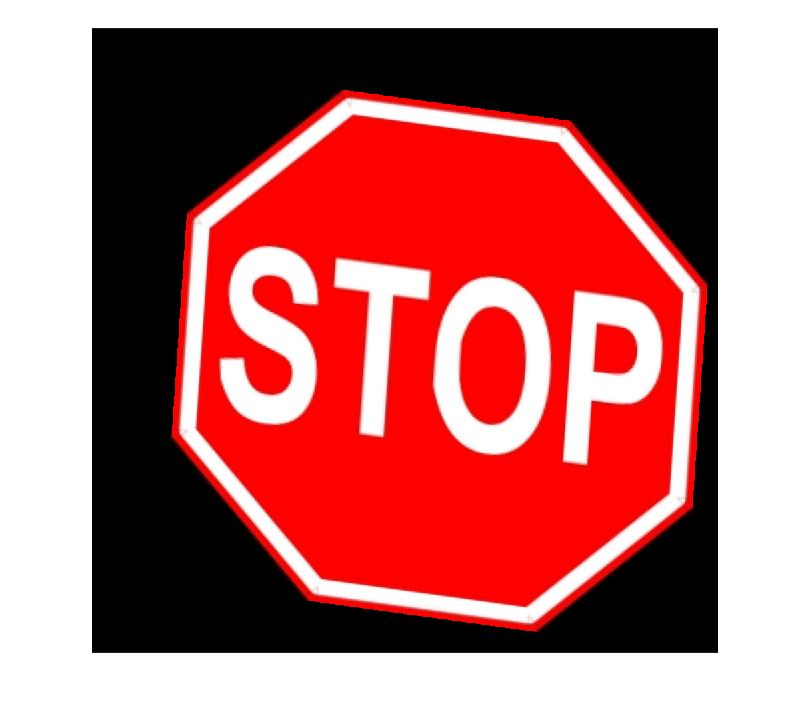
\includegraphics[width=\textwidth]{504.jpg}
		\caption{}
		\label{fig:504}
	\end{subfigure}
	
	\caption{Stop sign transformation from 1st image to all other images using the affine transformation.}
	\label{fig:500}
\end{figure}

\subsection{Step 6}

In this last step we stitched the projected sign from image 1 to the other images. We used NaN in projected pixels that don't appear in the first image, and we filtered out most of the black background of image 1 sign as well (for more accurate results, a mask of the stop sign can be used). Generally the sign was stitched well into the other images (not including lighting of course), but not perfectly as we can see best in Fig.~\ref{fig:604} where the affine transformation was insufficient in describing the projection (requiring perspective as well).

\begin{figure}[!htbp]
	
	\begin{subfigure}[b]{0.32\textwidth}
		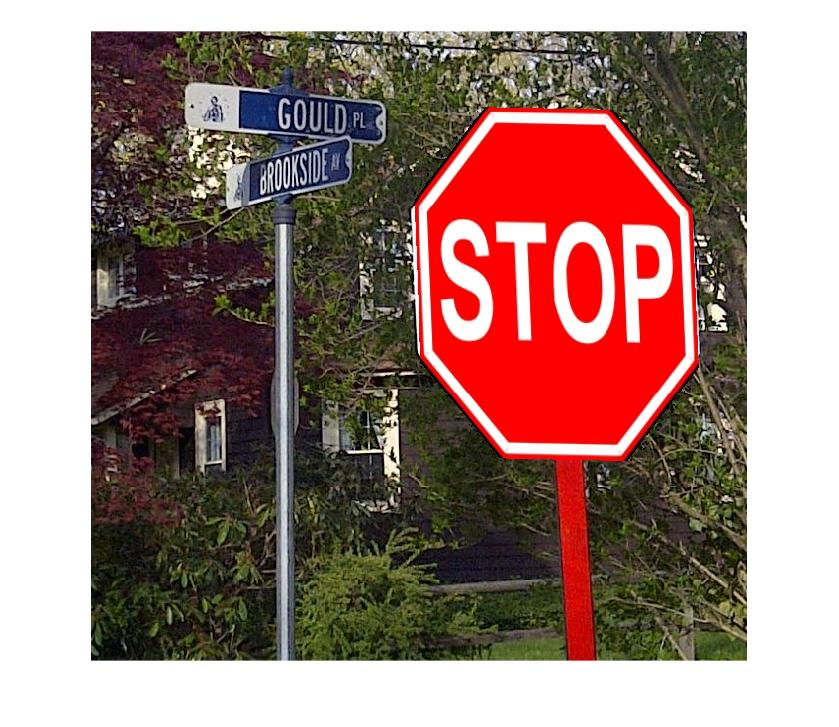
\includegraphics[width=\textwidth]{602.jpg}
		\caption{}
		\label{fig:602}
	\end{subfigure}
	%
	\begin{subfigure}[b]{0.32\textwidth}
		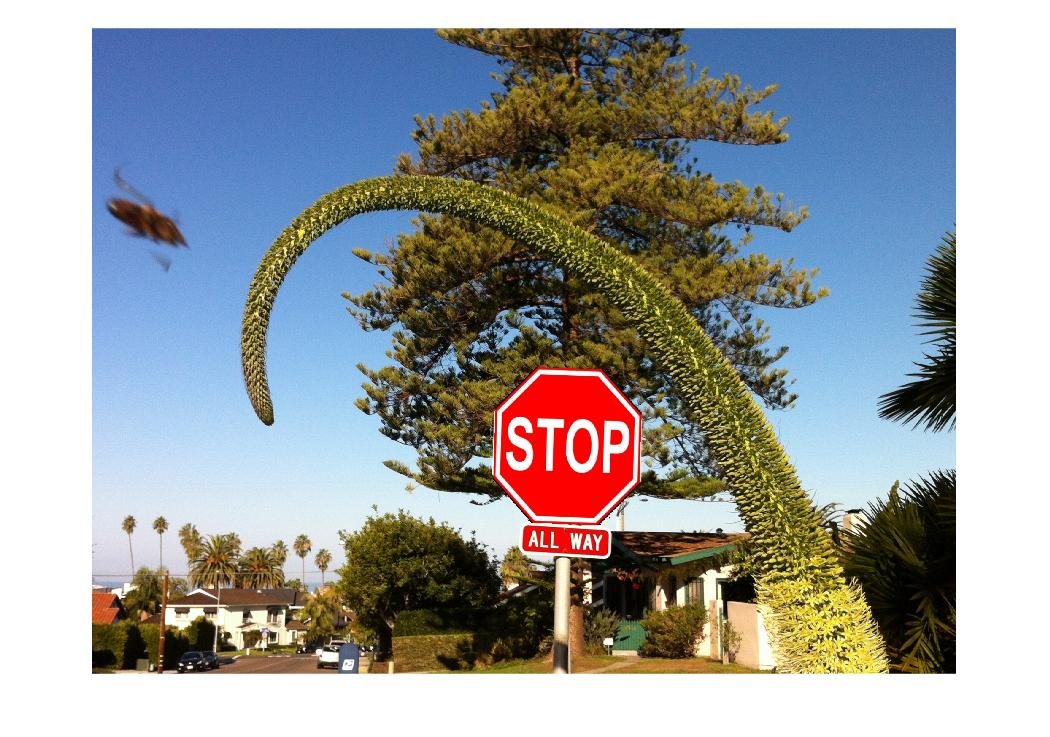
\includegraphics[width=\textwidth]{603.jpg}
		\caption{}
		\label{fig:603}
	\end{subfigure}
	%
	\begin{subfigure}[b]{0.32\textwidth}
		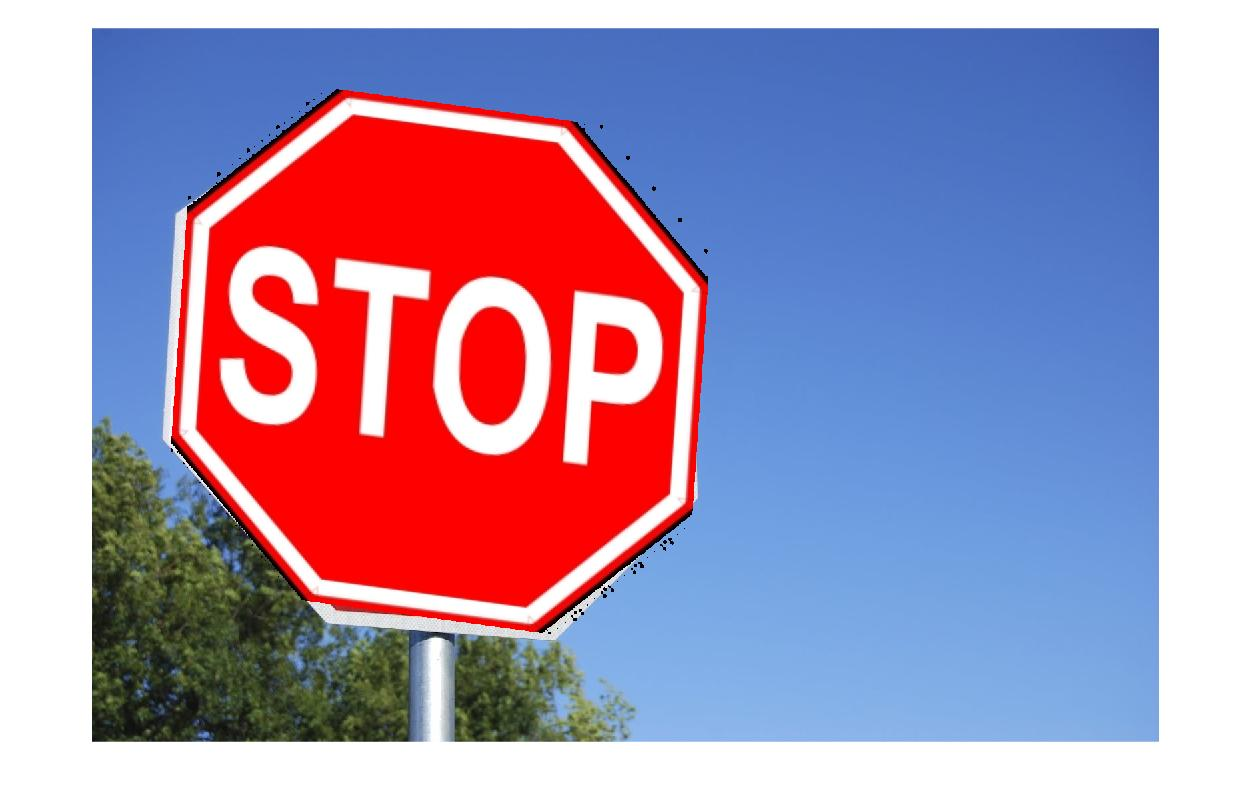
\includegraphics[width=\textwidth]{604.jpg}
		\caption{}
		\label{fig:604}
	\end{subfigure}
	
	\caption{Stop sign from the 1st image glued into all others.}
	\label{fig:600}
\end{figure}


\end{document}




